\section{Overbelægning}\label{sec:overbelaegning}

Overbelægning opstår, når der er flere patienter på en afdeling end der er normeret til\cite{Heidmann2014}. Dette sker ved akut indtag af uafviselige patienter. Herved overstiger antallet af patienter antallet af sengepladser, hvor det foruden at inddrage andre lokaler ligeledes bliver nødvendigt at anvende flugtvejsgange til patientophold(aftalevbrand). Når alle sengepladser på afdelingen er optaget, er kapaciteten på 100\%. I perioden fra år 1996 til 2011 er sengepladserne på de danske hospitalsafdelinger reduceret med 30 \%, hvilket kan have en betydning for antallet af disponible senge til akutte indlæggelser \cite{Madsen2014}. 

Antallet af akutte indlæggelser varierer hver måned, derfor vil tilgængeligheden af sengepladser ligeledes variere. Det fremgår af \figref{fig:overbelaegning_ran}, at overbelægning opstår på flere hospitalsafdelinger i Danmark. Ud af de 50 tilfældige hospitalsafdelinger har 35 af afdelingerne oplevet overbelægning i januar måned. Herudover fremgår det af figuren, at nogle afdelinger har haft en belægning på over 100\% op til 31 dage, hvilket svarer til, at afdelingen har haft overbelægning alle dage i januar måned. 


\begin{figure}[H]
	\flushleft 
	\caption{Overbelægning på 50 tilfældige hospitalsafdelinger i Danmark}
	\centering
	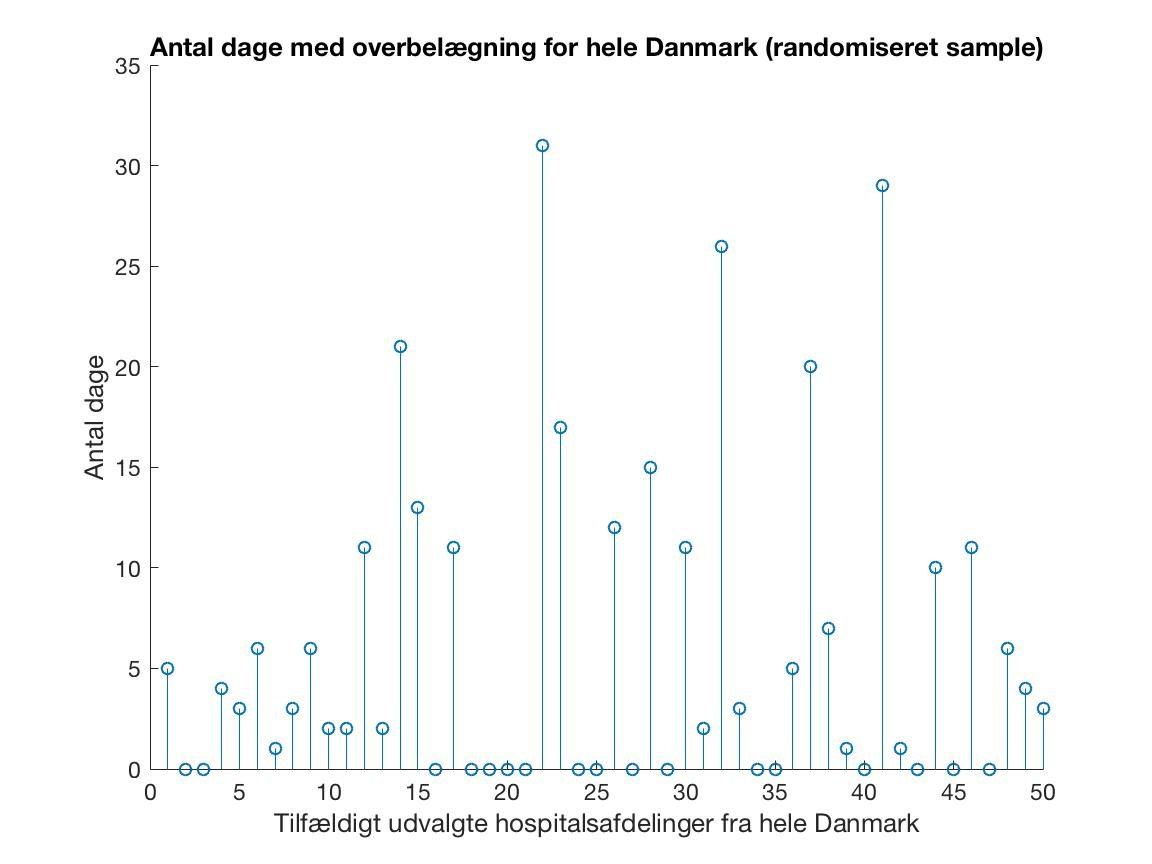
\includegraphics[scale=.3]{figures/overbelaegning_ran}
	\label{ig:overbelaegning_ran}
	\flushleft
	\textit{Illustrerer antal dage med overbelægning på 50 tilfældige hospitalsafdelinger fra hele Danmark. De tilfældige data er taget fra januar måned år 2015. \cite{SDS2015}}
\end{figure}



%\begin{figure}[H]
%\centering
%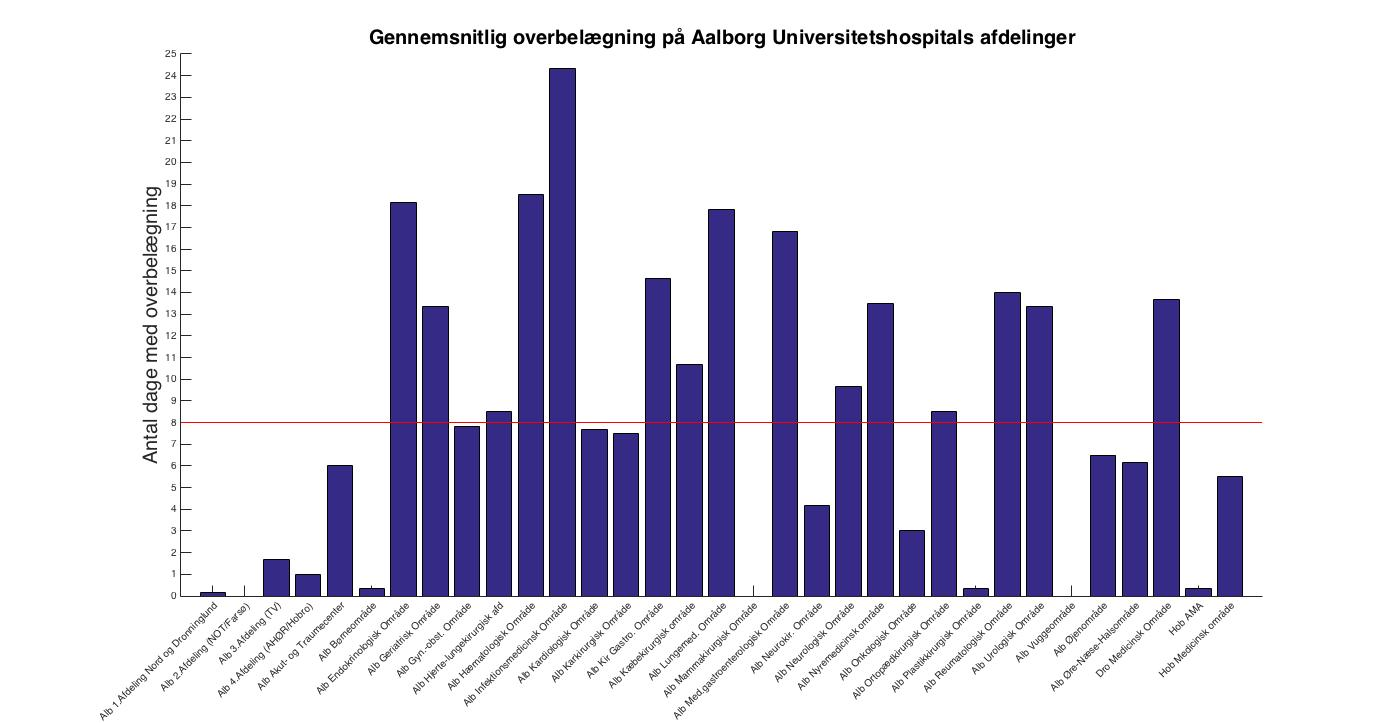
\includegraphics[width=1\textwidth]{figures/overbelaegning_AUH}
%\caption{Søjlerne illustrerer gennemsnittet af antal dage med overbelægning på Aalborg universitetshospitalsafdelinger fra januar til juni år 2015. \cite{SDS2015} Den røde linje viser gennemsnittet af søjlerne. Denne er beregnet til en gennemsnitlig overbelægning på 8,29 dage.}
%\label{fig:overbelaegning_AUH}
%\end{figure}

\noindent
Gennem de seneste år er Aalborg universitetshospitals opgave som akuthospital vokset, hvilket har resulteret i at patienttallet udfordrer de disponible sengepladser\cite{Handleplan2015}. Hertil har hospitalet i år 2016 haft fornyet fokus på at arbejde med sikkert patientflow samt at udnytte senge og ambulatorier effektivt for at patienter og personale skal undgå at opleve overbelægning samt for at undgå flaskehalse\cite{Handleplan2016}. Målet er at minimere patienternes ventetid, undgå unødige inlæggelser samt ambulante besøg\cite{Handleplan2016}. 

\noindent
I budgetfordelingen for Aalborg Universitetshospital i år 2017 indgår det, at ventetiden på en operation for elektive patienter skal reduceres fra 57 dage til 50 dage. \cite{Budget2016} Dette betyder optimering af planlægning ift. kapacitet. Dette skal ligeledes skabe et mere sammenhængende patientforløb og give bedre patientflow. Hertil kræves det, at tilgængelige ressourcer anvendes mest effektivt\cite{Handleplan2015}. Et større antal af elektive patienter kan dog mindske antallet af disponible sengepladser til akutte indlæggelser. 




%På \figref{fig:overbelaegning_ran} er det illustreret, hvordan de forskellige afdelinger  på tværs af Danmark oplever overbelægning i januar måned år 2015.

%\begin{figure}[H]
%\centering
%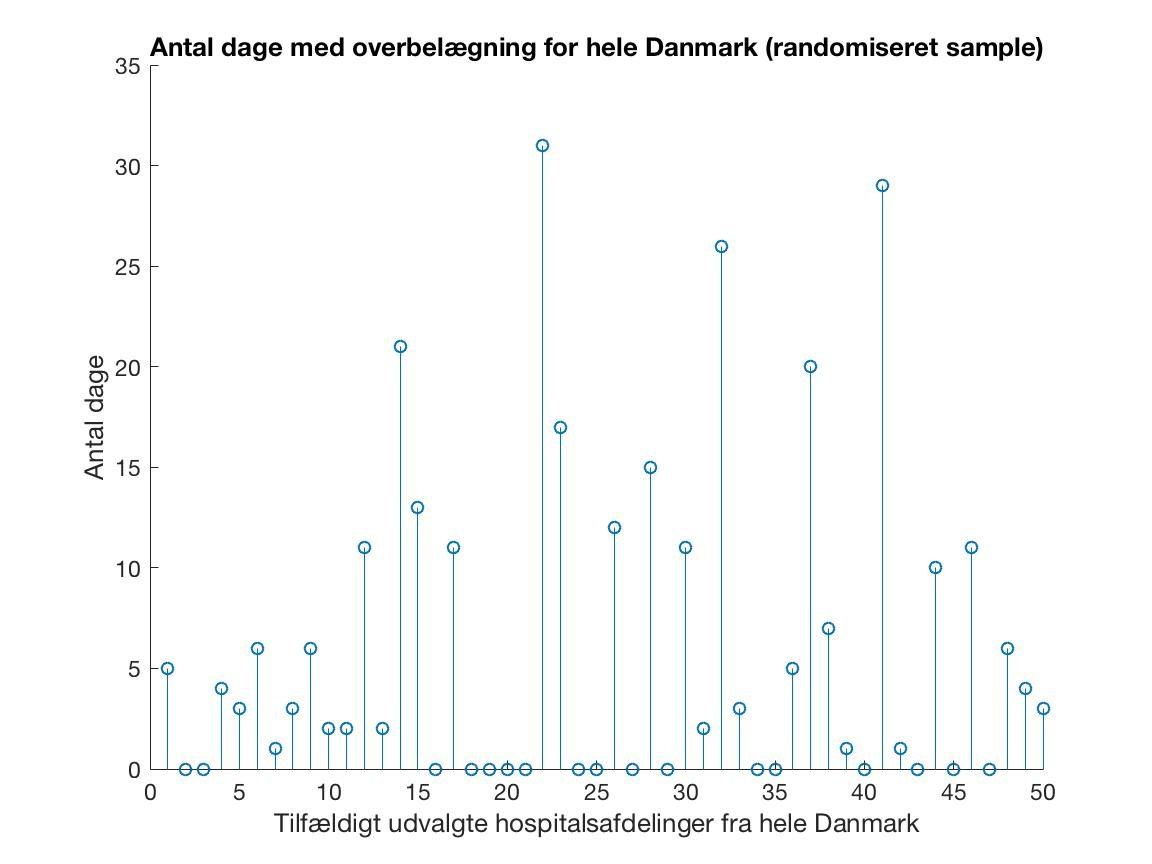
\includegraphics[width=1\textwidth]{figures/overbelaegning_ran}
%\caption{Illustrerer antal dage med overbelægning på 50 tilfældige hospitalsafdelinger fra hele Danmark. De tilfældige data er taget fra januar måned år 2015. \cite{SDS2015}} 
%\label{fig:overbelaegning_ran}
%\end{figure}

%Overbelægning opstår, når en afdeling har en belægningsprocent på over 85. I perioden fra år 1996 til 2011 er sengepladserne på de danske hospitalsafdelinger reduceret med 30 \%, for således at tilnærme sig en fuld udnyttelse af ressoucerne. Herunder udnyttelse af de tilgængelige sengepladser på hospitalsafdelingerne samt optimering af sundhedspersonalets arbejdstid \cite{Madsen2014}. 

%Antallet af indlagte patienter varierer hver måned, hvorfor tilgængeligheden af sengepladser ligeledes varierer. På \figref{fig:overbelaegning_ran} er det illustreret, hvordan de forskellige afdelinger  på tværs af Danmark oplever overbelægning i januar måned år 2015.


%Det fremgår af \figref{fig:overbelaegning_AUH}, at der ligeledes er en tendens til overbelægning på Aalborg universitetshospital. Der ses variation i antal dage med overbelægning på afdelingerne, dog ses overbelægning på 30 ud af 33 afdelinger i perioden fra januar til juni år 2015. På ambulatorisk infektionsmedicinsk område opleves en gennemsnitlig overbelægning på 24 dage, hvorimod eksempelvis ambulatorisk 2. afdeling ikke berøres af overbelægning. Gennemsnitlig er der en overbelægning på 8 dage for afdelingerne i perioden januar til juni år 2015.





